\chapter{Tests, conclusions and future work}

\section{Tests}
%% introduction and unit tests
Tests were carried out to understand how reliable the proposed solution is. Various techniques were used and the results are presented below. To begin with, various unit tests were performed on the exposed and unexposed methods of the application key store to reduce the number of errors in production and thus prevent the application key store from being unavailable for an edge case. During the first phase of testing, some errors were discovered. If these errors were not handled correctly, they led to crashes in the data store. For this, they have been fixed in various ways and modifications have been made: for example adding try catch blocks and failing safely in case an exception is raised. A problem that was discovered during this first phase of testing was the fact that it was initially possible to insert spaces within application names. It was already explained why it's a security issue and what an attacker can achieve by injecting a name with spaces inside the data store. To fix this issue, a check was inserted using the private function \textbf{appNameOk()}. Another problem found in this test phase concerns the public function \textbf{accessGranted()}. This function takes two strings as input: the name of an application and the authentication key. At first the logic of this method was only composed of the following line.
\begin{lstlisting}[language=java]
return keyStore.get(appName).equals(appKey);
\end{lstlisting}
If within the data store there is an entry with the name defined by appName, then the method correctly checks if the authentication key matches the one generated in the data store. The problem arises when an entry with the application name taken as input does not exist in the data store. In this case the \textbf{keyStore.get(appName)} method returns a null value, therefore the subsequent call to the \textbf{.equals(appKey)} method generates a NullPointerException exception which completely blocks the data store as it is not handled. As has already been shown previously in chapter 3, a check has been inserted to verify if there is an entry with the name of the specified application and if it does not exist, return the false value (access not granted). 
%% - test for errors
A data store is an important ONOS component for the security of the whole network environment (but not limited to network targets as already proved) and can be attacked as we have seen in previous chapters using many attacks, so it is crucial that many security tests are carried out. For this reason, tests were carried out that covered all the cases necessary to understand whether the application key store actually behaves correctly when an error should be raised. The correct handling of all error cases was not immediately implemented in the first version of the application key store, but during the entire research activity small proofs of concept were implemented to prove that there was actually a need to change some actions performed by the data store. In the first version created no tests were performed, while in the current version the tests carried out through malicious applications that exploited edge cases have produced various cases of error (and relative fixes):
\begin{itemize}
\item Malicious application tries to register with two names
\item Malicious application tries to guess the authentication key for another application
\item Malicious application tries to register using the name of a known application (e.g. ONOS default applications)
\item Malicious application tries to register with a name containing spaces (to then inject fake logs)
\end{itemize}
All of these cases have been handled either by implementing controls within the data store or by creating logs placed in the log file for Cross App Poisoning attacks which can be easily reviewed by the network operator.
\medskip

%% - produce a huge log file with more apps involved and more "active" data plane (add hosts and show how later, pingall from all the hosts, no hosts is changing location then y)
In addition to unit tests, additional tests were also carried out in a complete environment with a data plane. Of the various tests carried out, the one presented is the most recent, so that all the implemented functions are available. The test was performed with a modification of the malicious host tracking application presented in chapter 2. In particular when the application is started, it registers itself in the application key store and obtains the authentication credentials, then in order to create connection issues within the network, it changes the locations of random hosts every 500 milliseconds (swapping them by first adding new ones and then removing old ones). The test environment consists of an ONOS controller with active reactive forwarding application and other protocols and providers. Below is the output of the command \textbf{apps -a -s} in the ONOS shell showing the active applications.
\begin{lstlisting}
*   3 org.onosproject.hostprovider         2.7.0    Host Location Provider
*   4 org.onosproject.lldpprovider         2.7.0    LLDP Link Provider
*   5 org.onosproject.optical-model        2.7.0    Optical Network Model
*   6 org.onosproject.openflow-base        2.7.0    OpenFlow Base Provider
*   7 org.onosproject.openflow             2.7.0    OpenFlow Provider Suite
*  35 org.onosproject.drivers              2.7.0    Default Drivers
*  44 org.onosproject.gui2                 2.7.0    ONOS GUI2
*  74 org.onosproject.mal-host-tracking-app 2.7.0    Malicious Host Tracking Application
* 120 org.onosproject.fwd                  2.7.0    Reactive Forwarding
\end{lstlisting}
The proposed solution does not bind the network operator on any choice in the test phase. For example, multiple tests can be performed by choosing how the data plane must behave and what actions it performs. In the test carried out, no host has ever changed location (and this is used to carry out the test with the malicious host tracking application), but if the network operator deems it necessary, it is possible to carry out tests of this type. In the test carried out, the data plane consists of four switches to which four hosts with IP addresses starting from 10.0.0.1 up to 10.0.0.4 are connected. To make the data plane more dynamic, an initial \textbf{pingall} test was performed and then each host made ICMP echo connections to other hosts. It was not possible to use a python script that uses the Mininet API (due to an error it was not possible to connect the ONOS remote controller with the data plane), but it is an effective technique for programming the tests in a precise manner. Below it is presented a snippet that can be used in a real test; it performs three actions repetitively: (a) host H5 is created with IP address 10.0.0.5 and connected to the s4-eth3 interface of switch S4; (b) the newly created host makes ICMP connections, more precisely it sends an ICMP echo packet to every host present in the network; (c) host H5 is dropped from the network. Note how this test modifies the location of the hosts on the network using the APIs made available by ONOS.
\begin{lstlisting}[language=python]
def connTest(net):
    print( "Testing host connections" )
    while True:
        net.addHost('h5')
        s4 = net.get('s4')
        net.addLink(s4, net.get('h5'))
        s4.attach('s4-eth3')
        net.get('h5').cmd('ifconfig h5-eth0 10.0.0.5')

        # pingall
        net.get('h5').cmd('ping -c 1 10.0.0.1')
        net.get('h5').cmd('ping -c 1 10.0.0.2')
        net.get('h5').cmd('ping -c 1 10.0.0.3')
        net.get('h5').cmd('ping -c 1 10.0.0.4')
        
        # delete host
        net.delHost(net.get('h5'))
\end{lstlisting}
In the test performed the error catching functionalities were not tested, therefore no error log is present in the resulting file. After collecting the logs needed for the test, the python script was used to analyze the results. The file has been modified slightly to take an integer number as first parameter. This parameter determines the duration (in milliseconds) of the time section in which a potential Cross App Poisoning attack will be searched for. As example the number 5000 is used.
\begin{lstlisting}
$> python analyze-log.py 5000
\end{lstlisting}
The following shows the output produced by the python script in the terminal. The first section shows the edges of the graph built starting from the log file and their respective count. For example in this test the malicious application wrote 960 times to the data store host using the \textbf{appendLocation()} and \textbf{removeLocation()} APIs, while the reactive forwarding application read 417 times from the host data store (in this case using the \textbf{getHost()} API). The CAP attack vector found is the same as the attack already shown above: the malicious host tracking application writes to the host data store, then the reactive forwarding application reads from the host data store and finally writes to the flow rule data store. The APIs used to carry out the potential attacks are well known and the analysis concludes by telling the network operator that approximately nine thousand potential Cross App Poisoning attacks have been found. 
\begin{lstlisting}
---- edges ----
('org.edoardottt.malhosttracking.app', 'host')  :  960
('host', 'org.onosproject.fwd')  :  417
('org.onosproject.fwd', 'flow_rule')  :  90
('device', 'org.onosproject.test')  :  8

---- CAP gadgets ----
['org.edoardottt.malhosttracking.app', 'host', 'org.onosproject.fwd', 'flow_rule']

---- CAP gadgets APIs ----
[['appendLocation', 'removeLocation'], ['getHost'], ['forward']]

---- results ----
Found 9211 potentially exploited CAP attacks!
\end{lstlisting}

The figure 5.1 shows the resulting Cross App Poisoning attack vector graph produced by the python script. The test application logs were inserted in the log file in order to test also the analysis phase to check if Cross App Poisoning vectors are filtered correctly.
\begin{figure}[h]
\caption{Resulting test graph}
\label{fig:graphtest}
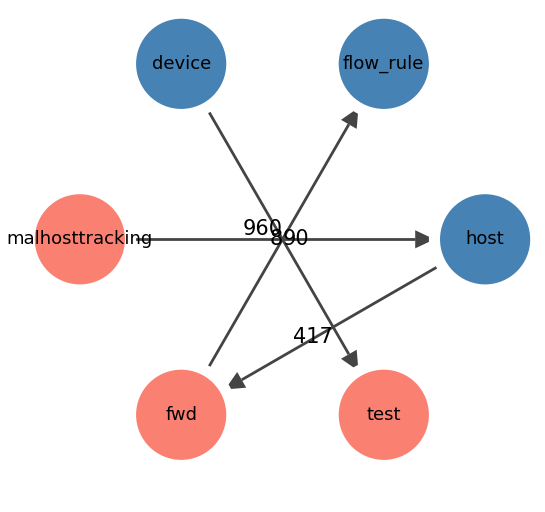
\includegraphics[width=1.0\textwidth]{resources/Chapter-5/graph1.png}
\centering
\end{figure}
%% - analysis on time section parameter in log analysis
The table 5.1 shows instead the results obtained by running the python script several times by changing the duration value of the time section. The tests carried out are ten and they have been numbered to discuss them more simply. The number 1 starts with a duration of 10000 milliseconds (or just 10 seconds) and the last one (the number 10) with a duration of a single millisecond. The table has four columns: the first indicates the test identification number, the second indicates the duration of the time section useful for identifying a potential Cross App Poisoning attack, the third indicates the number of potential Cross App Poisoning attacks found analyzing the log file, while the fourth is the execution time. It is interesting to note how much importance the duration value given to the time section has. This value significantly increases or decreases the number of potential findings. With a simple calculation we can figure out the number of Cross App Poisoning attacks actually carried out. We know that the malicious application wrote 960 times to the host data store. We also know that the malicious application uses exactly 4 API calls to perform a Cross App Poisoning attack (just because we have the source code, it would be slightly more complicated to reverse engineer and figure it out without the source code): two \textbf{appendLocation()} calls and two \textbf{removeLocation()} calls. So dividing the total number of calls made by the number of calls needed for an attack gives us the number of successful Cross App Poisoning attacks: $960 / 4 = 240$. Knowing this value makes more sense to think about the results obtained.
{\setlength{\extrarowheight}{5pt}%
\begin{table}[h]
\caption{Number of potential CAP attacks found in test log file}
\begin{tabular}{lllll}
\hline
\thead{N\#} & \thead{Time section (milliseconds)} & \thead{potential CAP attacks found} & \thead{Exec. time} \\ \cline{1-4}
\hline

\multicolumn{1}{l}{1} & \multicolumn{1}{l}{10000} & \multicolumn{1}{l}{26572} & \multicolumn{1}{l}{5.263378 sec.} \\ \cline{1-4}
\multicolumn{1}{l}{2} & \multicolumn{1}{l}{5000} & \multicolumn{1}{l}{9211} & \multicolumn{1}{l}{2.749676 sec.} \\ \cline{1-4}
\multicolumn{1}{l}{3} & \multicolumn{1}{l}{2000} & \multicolumn{1}{l}{2900} & \multicolumn{1}{l}{1.213360 sec.} \\ \cline{1-4}
\multicolumn{1}{l}{4} & \multicolumn{1}{l}{1000} & \multicolumn{1}{l}{1340} & \multicolumn{1}{l}{76 ms} \\ \cline{1-4}
\multicolumn{1}{l}{5} & \multicolumn{1}{l}{500} & \multicolumn{1}{l}{584} & \multicolumn{1}{l}{45 ms} \\ \cline{1-4}
\multicolumn{1}{l}{6} & \multicolumn{1}{l}{200} & \multicolumn{1}{l}{200} & \multicolumn{1}{l}{$< 2$ ms} \\ \cline{1-4}
\multicolumn{1}{l}{7} & \multicolumn{1}{l}{100} & \multicolumn{1}{l}{200} & \multicolumn{1}{l}{$< 2$ ms} \\ \cline{1-4}
\multicolumn{1}{l}{8} & \multicolumn{1}{l}{50} & \multicolumn{1}{l}{200} & \multicolumn{1}{l}{$< 1$ ms} \\ \cline{1-4}
\multicolumn{1}{l}{9} & \multicolumn{1}{l}{10} & \multicolumn{1}{l}{152} & \multicolumn{1}{l}{$< 1$ ms} \\ \cline{1-4}
\multicolumn{1}{l}{10} & \multicolumn{1}{l}{1} & \multicolumn{1}{l}{43} & \multicolumn{1}{l}{$< 1$ ms} \\ \cline{1-4}

\end{tabular}
\end{table}

% - final considerations
The first tests just make no sense because they are misleading looking at the results. Having a very large time section duration causes an excessively high number of logs to be counted as potential Cross App Poisoning attacks. On the contrary, a very small time section (such as in test \#10 with a time section lasting only one millisecond) could underestimate the number of Cross App Poisoning attacks actually carried out. Also looking at the execution time, we see that the longer the duration of the time section is, the longer the analysis takes.
\medskip

The tests prove that the proposed solution works correctly in many scenarios, even when malicious applications try to use the application key store and other implemented technologies in their favor. The output generated by the log file analysis can be modified according to the parameters that the network operator chooses as input. It is important to note that it will then be the same network operator who will check the suspicious sections of the log file to confirm the potential attacks resulting from the analysis (e.g. in this test no hosts changed location but the APIs related to the locations were used 960 times). In the last section possible future developments for the proposed solution will be presented and a discussion on how to improve the selection of the best duration for the time section used in log file analysis is included.

\clearpage

\section{Conclusions}
%% - problems with state of the art solutions
Before this new solution was proposed, there were two state-of-the-art defense tools against Cross App Poisoning attacks in Software Defined Networks: ProvSDN and vIFC. Actually the second uses the same technique as the first one with some improvements to better deal with certain situations, but in reality the defense methodology is the same. It has already been described why before implementing these solutions there must be set up a security policy regarding the access to the APIs offered by the controller, in particular the "least privilege" principle should be applied for better security and control of the actions available to the applications in the SDN environment. However, it has been widely shown that controlled access policy (or RBAC) alone cannot defend against Cross App Poisoning attacks due to their nature of API abuse in an indirect way. The methodology used in the two state-of-the-art solutions is an information flow control: an integrity value is assigned to each application through labels; based on which applications write or read these objects, the application integrity labels will influence the integrity value of the objects (data store). When the solution is activated, each API call is blocked before being completed and a provenance graph that traces the information flow is built. At each API call the graph is checked for possible policy violations (e.g. a Cross App Poisoning vector is present in the graph, the current API call is the last one in the path and the integrity label of the application trying to write is not compatible with the object which needs to be written). In case a policy violation is found, the API call can be blocked or a warning can be raised. The first solution implements the API blocking mechanism and the graph checks at the controller level, while the second one moves them in the data-plane level. The reason is that doing so is possible to enhance the previous solution to catch potential Cross App Poisoning attacks when virtual switches and/or multiple controllers are being used. 
\begin{itemize}
\item The biggest problem with these solutions is the integrity label system as already explained by the authors themselves. In the event that there are many deployed and active applications, the cases in which a legitimate application tries to write to an object with higher integrity and the API request is blocked may not be few and this limits by a lot the network capabilities.
\item The "self-revocation" problem is a method that could be exploited by an attacker to obtain advantageous results: if an application with a low-level integrity label writes to all objects it has access to, it successfully blocks access to higher integrity applications; in a nutshell, high-integrity applications will no longer be able to read from lower-integrity objects, only write to them.
\item The authors have performed many tests and compared to the baseline ProvSDN increases the time the controller takes for packet processing by a factor of 2x - 3x. In some types of networks where there are performance requirements, or simply in networks where many connections are made at the same time, this could be a very strong limitation. Even the authors recommend using the graph only when there are unusual changes of state and not always, but in doing so many attacks may not be detected. When vIFC (the second solution at state-of-the-art) is used, on average it is ten times slower than the baseline; that is an unacceptable defense method.
\item The vIFC authors suggest that an additional issue may arise if virtual switches become overwhelmed and vIFC could be unable to function properly, potentially allowing Cross Application Poisoning attacks to go unnoticed.
\item Not only switches or more generally network devices can be overwhelmed, but particularly in the case where applications require many permissions and therefore there is very loose role-based access control, the provenance graph would become an almost complete graph and this significantly increases the time it takes to figure out if a Cross App Poisoning attack in ongoing or not. In these cases, the capabilities and performance of a network are greatly reduced (whether the controller is being attacked or not).
\item In the event that an application is closed source and only the binary is available, a wrong information flow control policy could be created and therefore lead to security problems.
\end{itemize}
\medskip

%% - summary of the proposed solution
After discussing the limitations of current solutions, there are some important aspects that need to be addressed. Firstly, installing a new application is not a simple task and requires careful consideration. It is important to analyze the potential problems that may arise from a new network configuration. It is essential to have a solution that does not rely on source code or permissions lists and can be tested for Cross Application Poisoning attacks without affecting network performance. To address these issues, a new solution has been presented in this document. The idea is to conduct security tests offline, in an exact replica of the production environment, when a new application is installed. The network operator has full control over the tests that can be performed (connection tests; adding, removing or modifying devices and hosts...). This approach eliminates performance overhead, enables testing of compiled binaries that may not provide the necessary permissions list, and does not require an integrity label model. By testing applications in this way, network administrators can make informed decisions about which applications to install, ensuring the continued smooth operation of the network.

The proposed solution switches from a test method in production to one that uses a test environment. Considering the applications already present in the network as safe, a test environment is created with the same controller settings as the production environment, the new application is installed to be tested, while the data plane can (and is strongly recommended) be made dynamic and as more active as possible to test the functionalities of the application in as many scenarios as possible. The proposed solution adds a new data store for authenticating applications using the ONOS APIs. Applications must register themselves in this data store and by doing so they receive private authentication credentials. Whenever an application needs to use the ONOS APIs, it will do so by providing its authentication credentials. In case the credentials are correct, the API call is successful and all the necessary information is logged in a log file. Once all the tests have been performed the test environment is put down and an analysis is performed on the log file. This analysis builds a bipartite graph describing the APIs used throughout all the test duration. The Cross App Poisoning attack vectors present in the graph are then highlighted and the graph is scanned for all potential Cross App Poisoning attacks that may have been exploited in the testing phase. It is then up to the network operator to understand whether the sections of the log highlighted by the security analysis show a legitimate or malicious nature of the application being tested.
\medskip

%% - Results obtained
As shown in the previous section, many tests have been carried out and the entire research activity has led to the proposed solution which highlights many steps forward compared to the state of the art:
\begin{itemize}
    \item \texttt{The applications and network capabilities are not limited by an integrity label model}. In the test environment (and then also in production) applications can perform all the actions they want, this is essential both for malicious applications so that they show which methods they use to carry out the attacks, but above all for legitimate ones that obviously they must not be limited in their actions for the network to function correctly.
    \item \texttt{The network operator has complete control over the test environment}. In the test environment it is important that the controller settings and applications are copied from the production one to have tests that reflect as much as possible the ecosystem in which the tested application will then be installed. That said, the network operator has complete control over the test environment: different applications and settings can be used if they see fit. Beyond this, the data plane can be active and dynamic in order to best replicate real situations.
    \item \texttt{Minimal network overhead}. As already mentioned several times, there are network applications or entire ecosystems that require strict requirements. For example, an important requirement may be network performance and therefore latency overhead added by the security mechanism. In the proposed solution the production environment has minimum overhead since the only action that need to be performed is authentication, the graph creation and scanning is performed offline. In such scenario the systems that require real time capabilities can be safely tested.
    \item \texttt{Easy tracking and monitoring}. Even if only a compiled binary is distributed and therefore the network operator in this case has little information about the application to be installed, there is no need to define an information flow control policy. In addition, the proposed solution can easily trace and monitor all the actions performed by the application being tested, even for malfunctions, bugs, Cross App Poisoning attacks, but also security problems that go beyond the latter. For example, in the case of a loosely set role-based access control policy, it is still possible to trace the actions performed by the potentially malicious application and study its behavior for the entire test phase.
\end{itemize}

%% - minor results obtained
In addition to the results obtained through the study, implementation and testing of a new proposed solution, this research activity arrives at "minor" results which still give their contribution to literature and scientific research. First of all, CVE-2023-24279 was discovered, studied and proven to be an easily exploitable vulnerability with many results obtainable by an attacker. This vulnerability has remained unnoticed for more than six years. In addition to the vulnerability mentioned above, other security issues have been found in the latest version of ONOS (2.7.0 at the time of writing) and shown how they can be used by a potential attacker to gain advantage. For the first time, a Cross App Poisoning attack that has a different target than a network component or that affects the correct functioning of the network has been studied, implemented and tested. In particular, a Cross App Poisoning attack leading to a Cross Site Scripting attack was shown in the document. During the whole research activity, different attack attempts than the ones present in the literature have been studied, implemented and documented. In these cases not having a truly exploitable attack does not ensure that this is not possible or that these methods cannot be used in a larger and more complex attack. Several working attacks have been implemented and their source code is available online. These attacks can be improved by network and security researchers and investigated what other benefits a potential attacker could gain by making modifications. Finally, ideas for using data mining have been included in the document even though they are not used within the proposed solution. The next section discusses some ideas that could be improved in the future to achieve better results and which paths to follow to better study the problems addressed in this document.

\clearpage

\section{Future work}
%% - Introduction
This section aims to indicate what could be the paths to follow in the future to improve the proposed solution or better understand the whole study of Cross App Poisoning attacks and more generally the security in Software Defined Networks. It should be kept in mind that this document is a snapshot of a research activity that lasted several months. The future works presented in this section are techniques or improvements that have not found space in the time taken up to the writing of this document or attempts that have been made but have not led to satisfactory results. For this reason, researchers who want to work to advance the state of the art in the future can still study the attempts made in this research activity, conduct their own tests, obtain results and evaluate how these techniques can be used in other ways, which could potentially give satisfactory results.
\medskip

As already extensively explained in chapter 3 (Proposed Solution), the data store that is added in ONOS is a rather particular one since it does not support multiple ONOS nodes. The other data stores present (such as the Host data store, the flow rule data store or others encountered during the reading of this document) support data replication in multiple ONOS nodes. It was explained in Chapter 2 (System architecture and attack design) how data stores work and in particular how data is replicated across multiple copies of the same store. In order to support replications of the application key store in ONOS, solutions used by other stores should be implemented. For example, the data store should extend the AbstractStore abstract class, implement an interface that defines an application key store, and define a way to generate and handle events generated by the store. Doing so the proposed solution would have a much more reliable and secure data store, since the data is stored in multiple data stores and there is no single point of failure. As already explained above, in the event that the main ONOS node goes down or is no longer able to complete its actions, a replica node could become the main node and manage all the work of the network. Obviously this leads to the application key store and more generally the entire proposed solution being more tolerant to failures.
\medskip

In the implementation of the proposed solution, ONOS APIs that require authentication have been added to test whether this methodology can be a valid solution or not. Obviously this solution can be applied in a research environment, but not in a production business environment. To do this it is necessary to implement support for all the APIs offered by ONOS. By doing so all the APIs used by the applications will be logged in a log file and studied for Cross App Poisoning attacks. Also, the old ONOS APIs that didn't require authentication were still left available within ONOS to support other applications. In a real production environment the old APIs should not be exposed to force all applications to use the authentication method of the proposed solution.
\medskip 

%% - How the Log Analysis can be improved
In the document it was shown that once the logs describing the interactions between the applications and the controller (via authenticated APIs) have been collected, an analysis phase is performed on the resulting log file. This analysis phase can be divided into three macro sections: (a) construction of the bipartite graph of interactions between applications and data stores using the authenticated APIs; (b) search for Cross App Poisoning attack vectors; (c) search for potential exploited Cross App Poisoning attacks in the log file. In addition to the obvious improvements (such as improving the algorithms and data structures used throughout the entire process), changes could be made that would improve the experience of the security team or network operator. First, more control over the search for Cross App Poisoning attack vectors. In the current implementation, any path that could be exploited via a Cross App Poisoning attack is considered an exploitable vector. In reality, a network operator could choose to consider only those in which the new application being tested takes an active part in the process, or have a greater choice of available filters and, for example, accept only vectors that meet certain conditions. In chapter 3 (Proposed Solution) it was explained how some statistical data mining techniques were used to try to understand if through a log file the Cross App Poisoning attack vectors had been potentially exploited. As has already been widely explained, the log file was transformed from textual to numerical format and then two models were applied: Logistic Regression and K-nearest neighbors. Even if individually as models' score they did not perform badly, however they were not considered methods with suitable results for the detection of potential Cross App Poisoning attacks. Data mining techniques were not actually included in the proposed solution, but this does not exclude that they can be used if their effective utility is proven. For example, statistical techniques could be used alongside the scanning of the graph to confirm the results produced by the latter or could be used to tell how likely it is that a Cross App Poisoning attack vector found in the graph was actually used by an attacker by looking at the results of the analysis phase. 
\medskip

Another improvement that can be made is understanding which length of time section for log file analysis is most appropriate and produces the most reliable results in different network environments. For example, in networks where there are many applications installed, network devices such as switches and hosts are numerous and very active, it is very likely that many APIs will be used in a short time. This could mean that a shorter time section duration for graph analysis is more appropriate and may give more reliable results. Conversely, if fewer APIs are used, a longer time section duration could catch potential Cross App Poisoning attacks that took longer to complete. To obtain this result, specific analyzes through data mining are obviously not excluded. Obviously, if a researcher or a research team/laboratory wants to follow this research path and study possible methodologies, a lot of data and a lot of log files with different network characteristics must also be collected. It is useful to point out that the time section technique has been used to detect related API calls. In the examples that have been shown and used as tests it is assumed that the network is active, i.e. that hosts within the network perform connections with other hosts not rarely, but at a sustained pace. This feature means that when the malicious application actually starts the attack by calling an API with a malicious payload, the other actions take place within a limited section of time which then lead to the completion of the Cross App Poisoning attack. However, it should be noted that not all attacks are related to a time factor. For example, the attack targeting the ONOS Web application shown in chapter 4 (Security), might not be detected in a limited time section: the malicious application injects its malicious Javascript payload at time t. Then the network administrator might log into the web GUI application after a long time and therefore it isn't obvious that the Cross App Poisoning attack would be detected. Therefore, in view of these considerations, another modification that could bring improvements to the log file analysis system could be the distinction between Cross App Poisoning attack vectors which are linked to a time factor and others which are not. In this way the analysis of the graph would take into account the time factor only for the vectors in the first group, while for the others a scan of the entire log file is needed.
\medskip

%% - create standard mininet tests
Another improvement that could be studied and added to the proposed solution is a framework for standardizing tests via Mininet. Using this framework in addition to the Mininet API it could be possible to perform standard tests that every network must pass (such as connection tests or connection block tests where a firewall is present). Or, sticking to the examples given in this document, check that no hosts are relocated in a static network where no host is ever relocated within the network topology.
\medskip

%% - Continue the security vulnerability research
An important part of the activity was the vulnerability research in ONOS. The latter has led to excellent results: more than one security vulnerability found and truly exploitable and the study and proof of concept implementation of the first Cross App Poisoning attack that targets a Web component. Other paths followed in the activity have turned out to be blind spots, such as the implementation of an application that uses events and event listeners to carry out a Cross App Poisoning attack, or the implementation of an attack that through the manipulation of host locations obtains port mirroring (an host compromised by an attacker could receive network packets intended for the victim). To continue the study carried out in this research activity, these failed attempts could be revised, correcting the errors if possible and obtaining satisfactory results. As already mentioned, the objectives that had been designated in this document do not necessarily have to remain the same: for example, studies on failed attempts could lead to more complex attacks that require the addition of other components or techniques. However studies on how to use Cross App Poisoning attacks in new scenarios or using new techniques would in any case add something to the state of the art.


\clearpage